\cleardoublepage % memastikan bab baru dimulai di halaman ganjil (kanan)
\chapter{PENDAHULUAN}
\label{chap:pendahuluan}
% --- Latar Belakang ---
\section{Latar Belakang}
Berdasarkan Kamus Besar Bahasa Indonesia (KBBI), tiket atau karcis adalah surat kecil (carik kertas khusus) sebagai tanda telah membayar ongkos dan sebagainya (untuk naik bus, menonton bioskop, dan sebagainya). Tiket merupakan sebuah dokumen yang berfungsi sebagai bukti hak akses atau tanda pembayaran yang sah untuk menggunakan suatu layanan atau memasuki suatu area tertentu. Secara historis, tiket konvensional dalam bentuk fisik telah menjadi bagian tak terpisahkan dari berbagai sektor, mulai dari transportasi hingga hiburan. Namun, seiring dengan pesatnya perkembangan teknologi informasi, terjadi pergeseran paradigma menuju digitalisasi tiket menjadi tiket elektronik (\textit{e-ticket}). Inovasi sistem pertiketan ini sangat erat kaitannya dengan adopsi sistem teknis berbasis komputer yang memungkinkan peningkatan efisiensi dan efektivitas operasional \cite{lubeck2012electronic}. Pergeseran paradigma tersebut didorong oleh kebutuhan untuk meningkatkan manajemen informasi yang sebelumnya sulit dilakukan dengan sistem manual atau kartu magnetik \cite{lubeck2012electronic}. 

Adopsi \textit{e-ticket} mulai marak pada awal tahun 2000-an, yang dipelopori oleh industri penerbangan di tahun 1990-an, dan kini telah diadopsi secara masif di berbagai sektor. \textit{E-ticket} menawarkan berbagai keunggulan signifikan dibandingkan tiket konvensional yang rentan terhadap inefisiensi. \textcite{lubeck2012electronic} menyoroti bahwa sistem konvensional seringkali terkendala oleh lemahnya kontrol operasional yang menyebabkan maraknya perdagangan tiket ilegal serta penyalahgunaan manfaat tiket khusus (seperti tiket pelajar) karena sulitnya identifikasi pengguna. Dari sisi pengguna, \textit{e-ticket} memberikan kemudahan distribusi dan akses, menghilangkan risiko kehilangan tiket fisik, serta membantu menghindari antrean panjang. Selain itu, infrastruktur digital ini juga lebih efisien dari segi biaya operasional karena mengurangi penggunaan kertas dan menghindari komisi yang dibayarkan kepada sistem distribusi dan agen \cite{chen2007passenger}.

Secara operasional, implementasi \textit{e-ticket} dalam manajemen acara berskala besar umumnya terbagi menjadi dua model pemenuhan akses (\textit{access fulfillment}) [Perlu Sitasi: Jurnal/prosiding terkait proses bisnis pertiketan acara atau manajemen kontrol akses acara (misal: \textit{Event Access Control Systems} / \textit{E-ticket Lifecycle Management})]. Model pertama adalah penukaran fisik (\textit{voucher redemption}), di mana bukti pembelian digital harus ditukarkan terlebih dahulu dengan medium fisik sekunder, seperti gelang berbasis \textit{Radio Frequency Identification} (RFID) atau tiket kertas khusus di lokasi acara sebelum penonton dapat memasuki gerbang utama [Perlu Sitasi: Artikel/studi kasus manajemen tiket konser/festival yang menggunakan sistem penukaran fisik atau gelang RFID]. Meskipun menawarkan tingkat keamanan fisik yang baik, model ini menimbulkan inefisiensi baru berupa penumpukan antrean ganda pada loket penukaran dan pembengkakan biaya produksi perangkat keras [Perlu Sitasi: Jurnal mengenai analisis antrean atau efisiensi biaya pada penukaran tiket fisik]. Oleh karena itu, industri hiburan kini bergeser menuju model kedua, yaitu akses digital langsung (\textit{direct digital access}). Pada model ini, kredensial elektronik yang diterima pengguna di ponsel pintar mereka berfungsi langsung sebagai token akses akhir yang divalidasi di gerbang masuk, meniadakan kebutuhan perantara medium fisik sama sekali [Perlu Sitasi: Jurnal/artikel tentang tren \textit{digital ticketing} dan \textit{paperless access control}].

Untuk merealisasikan efisiensi pada model akses digital langsung tersebut, diperlukan medium representasi data yang ringan, efisien, dan kompatibel dengan perangkat pengguna. Di antara berbagai alternatif teknologi, \textit{Quick Response Code} (QR Code) muncul sebagai solusi dominan yang diadopsi secara luas dalam implementasi \textit{e-ticket}. QR Code adalah jenis kode batang (\textit{barcode}) matriks atau kode dua dimensi yang dapat menyimpan informasi digital \cite{shin2012psychology}. Tidak seperti \textit{barcode} satu dimensi, QR Code mengenkode data secara horizontal dan vertikal, menawarkan kepadatan informasi yang lebih tinggi dan kecepatan pembacaan yang lebih cepat \cite{alsuhibany2025innovative}. \textcite{tiwari2016introduction} menjelaskan bahwa tingkat penerimaan QR Code yang tinggi secara global berbanding lurus dengan pertumbuhan pengguna ponsel pintar, yang memungkinkan teknologi ini menjangkau konsumen secara luas dan cepat. Ubikuitas perangkat pemindai yang terintegrasi dalam ponsel pintar menjadikan QR Code pilihan yang praktis dan efisien untuk diterapkan sebagai medium \textit{e-ticket}. Kepopuleran dan kemudahan akses tersebut mendorong adopsi luas QR Code pada gerbang transportasi maupun acara hiburan. Akan tetapi, model \textit{e-ticket} generasi awal yang mengandalkan representasi kode QR statis secara inheren mewarisi celah keamanan yang sangat serius.

Sistem \textit{e-ticket} generasi awal pada umumnya mengadopsi model kode QR statis [Perlu Sitasi: Artikel/jurnal pendukung terkait dominasi arsitektur kode QR statis pada generasi awal \textit{mobile ticketing}]. Pada model ini, data tiket seperti identitas pengguna atau tautan validasi, dienkode secara langsung ke dalam pola matriks citra. Karakteristik fundamental dari kode QR statis adalah informasi yang tersimpan di dalamnya bersifat tetap (\textit{fixed information}) \cite{yanuarafi2023perbandingan}; artinya, setelah kode dibangkitkan (\textit{generated}), pola visualnya tidak akan berubah dan terus valid sepanjang masa berlaku tiket. Proses validasi bergantung sepenuhnya pada pemindaian di pintu masuk, yaitu saat alat pemindai menerjemahkan kembali pola matriks menjadi data identitas untuk dicocokkan dengan basis data. Meskipun arsitektur ini menawarkan kemudahan implementasi, menurut \textcite{yanuarafi2023perbandingan}, penggunaan kode QR statis memiliki kelemahan signifikan dalam aspek keamanan. Sifatnya yang permanen membuat sistem ini rentan terhadap penyalahgunaan, seperti duplikasi ilegal dan pemalsuan, yang pada akhirnya mengancam integritas ekosistem \textit{e-ticket} secara keseluruhan.

Kelemahan mendasar dari arsitektur statis adalah sifatnya yang ``sekali terbit, berlaku selamanya'' tanpa mekanisme pembaruan autentikasi. Celah tersebut dieksploitasi secara luas melalui serangan penggandaan (\textit{cloning}) dan serangan putar ulang (\textit{replay attack}). \textcite{sung2015security} dalam analisis keamanannya menegaskan bahwa kode QR sangat mudah diduplikasi melalui fitur tangkapan layar (\textit{screen capture}) pada perangkat seluler, yang kemudian dapat ditransfer ke pihak lain tanpa bisa dicegah oleh sistem konvensional. Dampak dari kerentanan ini menciptakan efek domino kerusakan pada ekosistem pertiketan. 

Pertama, pada aspek validasi di lapangan, insiden konser Coldplay di Jakarta tahun 2023 memperlihatkan kekacauan di pintu masuk ketika banyak pemegang tiket sah gagal mendapatkan akses karena tiket mereka telah digandakan dan digunakan lebih dulu oleh pihak lain. Berdasarkan analisis hukum, modus ini terjadi karena pelaku mempelajari desain visual tiket statis lalu menggandakannya untuk dijual ke banyak korban \cite{berma2023analisis}. Kedua, lemahnya sistem keamanan turut menyuburkan praktik percaloan (\textit{scalping}), yaitu dengan menjual kembali tiket yang telah dibeli secara legal dengan harga berkali-kali lipat dari harga resmi sehingga merusak kewajaran pasar \cite{Pamela2023}. Ketiga, kegagalan kontrol akses berlanjut hingga ke dalam arena, seperti pada salah satu pertandingan Timnas Indonesia di Gelora Bung Karno (GBK). Pada kasus tersebut, penonton tanpa hak akses valid berhasil masuk dan menduduki kursi pemegang tiket sah, memicu konflik fisik dan ketidaknyamanan \cite{Kurniawan2024}. Terakhir, dari sisi kerugian materiil, investigasi Kompas mengungkapkan data Pusat Pelaporan dan Analisis Transaksi Keuangan (PPATK) yang mencatat 182 kasus transaksi mencurigakan terkait penipuan tiket konser pada tahun 2024 dengan total nilai Rp 2,3 miliar \cite{diveranta2025jejak}. Rangkaian kasus ini menegaskan bahwa arsitektur statis gagal memberikan perlindungan menyeluruh, baik dari sisi keamanan akses, keadilan harga, maupun perlindungan hak konsumen.

Kompleksitas permasalahan tersebut membuktikan bahwa verifikasi berbasis kode QR statis tidak lagi memadai. Sebagai respons, industri mulai beralih pada arsitektur tiket dinamis menggunakan algoritma \textit{Time-based One-Time Password} (TOTP) yang membatasi masa berlaku visual tiket dalam hitungan detik \cite{sung2015security}. Namun, pengamanan data tiket secara dinamis ini belum menyelesaikan tantangan operasional terbesar dalam acara berskala masif: risiko ketergantungan penuh pada konektivitas internet ke server pusat, atau dikenal sebagai Titik Kegagalan Tunggal (\textit{Single Point of Failure}). Kerentanan ini terbukti dari insiden kendala teknis pada \textit{platform} Ticketmaster saat lonjakan penjualan tiket konser \cite{cockroach2023taylor} serta kegagalan berantai pada infrastruktur awan akibat malfungsi satu layanan inti \cite{aws2017summary}. Jika server validasi tiket mengalami gangguan serupa saat acara berlangsung, alat pemindai di lokasi akan kehilangan fungsinya dan memicu kemacetan fatal di gerbang masuk. Oleh karena itu, pemindai gerbang harus mampu memvalidasi tiket secara mandiri (\textit{offline validation}) menggunakan manajemen penyimpanan lokal (\textit{local cache}).

Ironisnya, penerapan validasi \textit{offline} yang dikombinasikan dengan algoritma TOTP standar membuka sebuah celah keamanan baru yang fatal, yaitu serangan penggandaan multi-gerbang (\textit{Multi-Gate Cloning}) [Perlu Sitasi: Jurnal/makalah keamanan sistem mengenai celah replikasi/penyusupan simultan pada token berbasis waktu pada arsitektur terdistribusi tanpa koneksi \textit{real-time}]. Jika seorang pelaku menduplikasi aplikasi atau kredensial tiket dan memberikannya kepada orang lain, kedua tiket identik tersebut dapat digunakan secara bersamaan di dua gerbang masuk yang berbeda. Karena kedua perangkat pemindai beroperasi tanpa terhubung ke basis data pusat secara \textit{real-time}, dan algoritma TOTP hanya bergantung pada parameter waktu universal, sistem pada kedua gerbang akan menganggap kedua tiket tersebut valid. Kondisi ini memperlihatkan bahwa pembatasan waktu saja tidak cukup untuk menjamin keunikan akses pada lingkungan banyak gerbang (\textit{multi-gate}) dalam keadaan luring.

Oleh karena itu, diperlukan sebuah kebaruan (\textit{novelty}) dalam arsitektur kriptografi tiket untuk memitigasi serangan multi-gerbang secara \textit{offline}. Penelitian ini mengusulkan pengembangan sistem \textit{Dynamic Secure QR Code} yang mengintegrasikan Tanda Tangan Digital berbasis \textit{Elliptic Curve Digital Signature Algorithm} (ECDSA), prinsip \textit{Data Minimization}, dan algoritma \textit{Gate-Bound TOTP} berbantuan teknologi \textit{Bluetooth Low Energy} (BLE). Melalui pemanfaatan BLE, perangkat pemindai pada setiap gerbang akan bertindak sebagai \textit{beacon} yang memancarkan identitas gerbang secara lokal [Perlu Sitasi: Jurnal/referensi standar pemanfaatan \textit{BLE beacon} untuk pembatasan spasial / \textit{proximity-based authentication}]. Aplikasi pada ponsel pengguna kemudian menangkap sinyal kedekatan (\textit{proximity}) ini dan menginjeksikannya sebagai parameter tambahan dalam pembangkitan kode TOTP. Mekanisme ini memastikan bahwa kode QR yang dibangkitkan tidak hanya dinamis terhadap waktu, tetapi juga terkunci secara spasial pada gerbang spesifik, mematikan celah penyusupan ganda meskipun sistem beroperasi sepenuhnya dalam mode \textit{offline}.

% --- Rumusan Masalah ---
\section{Rumusan Masalah}
Berdasarkan latar belakang yang telah diuraikan, teridentifikasi bahwa kombinasi QR Code dinamis (TOTP) dan mekanisme validasi luring (\textit{offline}) pada sistem \textit{e-ticket} generasi awal masih memiliki celah keamanan fatal berupa serangan penggandaan multi-gerbang (\textit{multi-gate cloning}). Oleh karena itu, rumusan masalah dalam penelitian ini adalah sebagai berikut:
\begin{enumerate}
    \item Bagaimana merancang arsitektur sistem \textit{Dynamic Secure QR Code} yang mengintegrasikan Tanda Tangan Digital (ECDSA) dan prinsip \textit{Data Minimization} untuk memastikan keaslian penerbit tiket sekaligus mencegah kebocoran data pribadi pengguna?
    \item Bagaimana mengembangkan mekanisme validasi luring (\textit{offline validation}) yang kebal terhadap serangan penyusupan multi-gerbang menggunakan modifikasi algoritma \textit{Gate-Bound TOTP} berbantuan teknologi \textit{Bluetooth Low Energy} (BLE)?
    \item Bagaimana menjaga konsistensi data riwayat pemindaian tiket antara perangkat pemindai lokal dan basis data server pusat (\textit{cloud}) tanpa mengorbankan kecepatan operasional gerbang masuk?
\end{enumerate}

% --- Tujuan ---
\section{Tujuan Penelitian}
Mengacu pada rumusan masalah di atas, tujuan utama dari penelitian ini adalah:
\begin{enumerate}
    \item Merancang dan mengimplementasikan arsitektur sistem \textit{e-ticket} berlapis yang memanfaatkan algoritma Tanda Tangan Digital (ECDSA) dan \textit{Data Minimization} untuk menjamin integritas data serta melindungi privasi penonton.
    \item Mengembangkan mekanisme validasi \textit{offline} yang tangguh dengan mengintegrasikan algoritma \textit{Gate-Bound TOTP}, di mana perangkat pemindai memancarkan sinyal BLE (\textit{beacon}) untuk mengunci validitas token secara spasial pada gerbang spesifik, mematikan ancaman \textit{multi-gate cloning}.
    \item Menerapkan mekanisme sinkronisasi data asinkron (\textit{batching}) untuk menjaga konsistensi dan integritas status penggunaan tiket antara penyimpanan lokal aplikasi pemindai dan server pusat secara efisien.
\end{enumerate}

% --- Batasan Masalah ---
\section{Batasan Masalah}

Agar pengerjaan tugas akhir dapat lebih terarah dan tidak melenceng dari tujuan utamanya, ruang lingkup permasalahan dibatasi sebagai berikut:
\begin{enumerate}
    \item Penelitian ini berfokus pada perancangan dan implementasi modul inti keamanan, yaitu proses pembangkitan (\textit{generation}) dan validasi (\textit{validation}) \textit{Dynamic Secure QR Code}, tanpa membahas aspek antarmuka pengguna (UI/UX) secara mendalam.
    \item Penelitian ini tidak mencakup pengembangan fitur sistem penjualan tiket yang kompleks (seperti integrasi gerbang pembayaran atau manajemen kursi acara), melainkan murni berfokus pada siklus hidup keamanan tiket elektronik.
    \item Luaran sistem yang dibangun berupa prototipe (\textit{proof-of-concept}) Minimum Viable Product (MVP) yang bertujuan untuk mendemonstrasikan kelayakan logika keamanan secara terdistribusi (\textit{mobile} dan \textit{backend cloud}), bukan aplikasi komersial.
    \item Sistem menerapkan prinsip \textit{Data Minimization}, di mana muatan data (\textit{payload}) QR Code hanya berisi atribut teknis non-sensitif. Data identitas pribadi pengguna (PII) tetap disimpan di server.
    \item Penelitian ini tidak menggunakan perangkat keras \textit{beacon} BLE eksternal atau khusus. Sebagai bentuk efisiensi operasional, fungsi pemancar (\textit{broadcaster}) identitas gerbang dieksekusi langsung secara perangkat lunak menggunakan modul \textit{Bluetooth} bawaan pada ponsel pintar (\textit{smartphone}) bersistem operasi Android yang digunakan oleh petugas pemindai.
    \item Perangkat pemindai diasumsikan sebagai perangkat terpercaya (\textit{trusted device}) yang memiliki mekanisme keamanan fisik memadai. Risiko eksfiltrasi (\textit{Master Secret}) dari perangkat petugas melalui (\textit{reverse engineering}) berada di luar lingkup penelitian.
    \item Isu sinkronisasi data secara \textit{real-time} (\textit{peer-to-peer}) antar-banyak pemindai dalam kondisi \textit{offline} penuh tidak dibahas, karena sistem mengandalkan validasi kriptografis dan BLE untuk menyelesaikan masalah sinkronisasi tersebut.
\end{enumerate}

% --- Metodologi ---
\section{Metodologi}
Pengerjaan tugas akhir ini menerapkan kerangka kerja \textit{Software Development Life Cycle} (SDLC) dengan pendekatan model \textit{Waterfall} sebagai metodologi. Model ini dipilih karena kebutuhan sistem (\textit{requirements}) telah terdefinisi secara jelas sejak tahap awal, yang berfokus pada modifikasi algoritma keamanan QR Code. Tahapan pengembangan sistem mengacu pada standar rekayasa perangkat lunak menurut \textcite{sommerville2016software}, yang visualisasinya dapat dilihat pada Gambar \ref{fig:metodologi_waterfall}.

\begin{figure}[h]
    \centering
    \captionsetup{justification=centering}
    	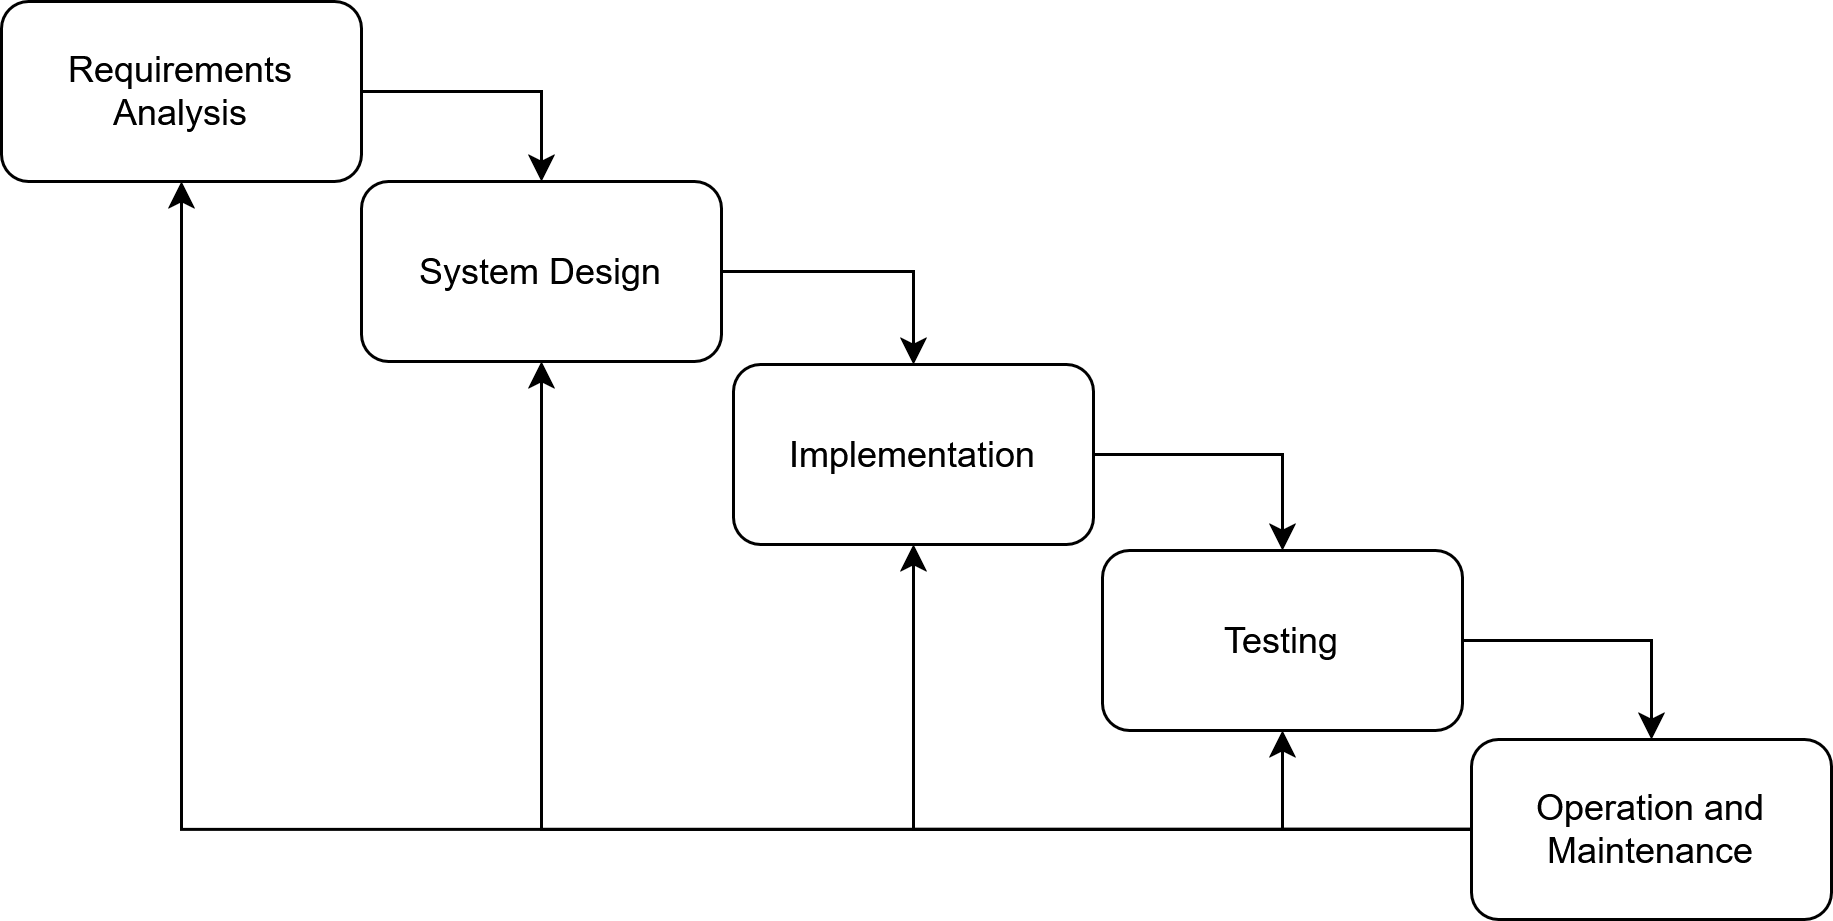
\includegraphics[width=0.9\textwidth]{images/waterfall.png}
    \caption{Alur Metodologi Penelitian Model Waterfall}
    \label{fig:metodologi_waterfall}
\end{figure}

Rincian tahapan yang dilalui selama pelaksanaan tugas akhir adalah sebagai berikut:

\begin{enumerate}
    \item \textbf{Analisis Kebutuhan (\textit{Requirements Analysis})} \\
    Tahapan fundamental untuk mengumpulkan fakta empiris terkait fenomena kelumpuhan validasi gerbang luring (\textit{offline}) dan serangan \textit{multi-gate cloning}. Selain itu, dilakukan studi literatur terhadap kriptografi asimetris (ECDSA), algoritma TOTP, serta spesifikasi protokol \textit{Bluetooth Low Energy} (BLE) sebagai landasan teoretis untuk pengembangan solusi.

    \item \textbf{Perancangan Sistem (\textit{System Design})} \\
    Spesifikasi kebutuhan diterjemahkan menjadi representasi desain arsitektur berlapis. Perancangan mencakup desain algoritma \textit{Key Derivation Function} (KDF), skema injeksi \textit{payload} sinyal BLE ke dalam parameter perhitungan TOTP (\textit{Gate-Bound}), serta perancangan model sinkronisasi data asinkron (\textit{batching}) antara \textit{local cache} dan \textit{cloud database}.

    \item \textbf{Implementasi (\textit{Implementation})} \\
    Tahap merealisasikan rancangan menjadi unit program fungsional. Implementasi dibagi menjadi dua sisi: \textit{Backend} (dikembangkan menggunakan FastAPI untuk manajemen penerbitan dan ECDSA \textit{Signature}) dan Klien \textit{Mobile} (dikembangkan menggunakan React Native untuk integrasi modul pemindai, antarmuka penonton, dan pemancar BLE \textit{native}).

    \item \textbf{Pengujian (\textit{Testing})} \\
    Tahap verifikasi dan validasi keandalan prototipe sistem. Pengujian berfokus pada \textit{Security Testing} secara \textit{Black Box} yang mencakup simulasi skenario ekstrem seperti upaya modifikasi muatan tiket, pemindaian tiket kedaluwarsa, hingga percobaan akses ganda (\textit{cloning}) pada kondisi gerbang luring sesungguhnya.

    \item \textbf{Operasi dan Pemeliharaan (\textit{Operation and Maintenance})} \\
    Dalam konteks tugas akhir, tahapan ini dialihfungsikan menjadi fase penyusunan dokumentasi dan pelaporan akhir. Artefak pengembangan dievaluasi untuk menarik kesimpulan yang menjawab rumusan masalah.
\end{enumerate}

% --- Sistematika Penulisan ---
\section{Sistematika Penulisan}
Untuk mempermudah pemahaman alur pembahasan, laporan tugas akhir ini disusun secara sistematis ke dalam tujuh bab utama dengan rincian sebagai berikut:

\begin{enumerate}
\item	\textbf{Bab I Pendahuluan} \\
Bab ini mendeskripsikan latar belakang permasalahan kerentanan pada sistem \textit{e-ticket}, rumusan masalah, tujuan penelitian, batasan masalah, metodologi pengembangan perangkat lunak yang digunakan, serta sistematika penulisan laporan.
\item	\textbf{Bab II Studi Literatur:} \\
Bab ini memaparkan landasan teoretis dan kajian pustaka terdahulu yang mendukung penyelesaian masalah. Topik yang dibahas meliputi konsep manajemen \textit{e-ticket}, \textit{Quick Response (QR) Code}, kriptografi kunci publik dan Tanda Tangan Digital (ECDSA), derivasi kunci (HMAC), algoritma \textit{Time-based One-Time Password} (TOTP), serta dasar teknologi komunikasi \textit{Bluetooth Low Energy} (BLE).
\item	\textbf{Bab III Analisis Masalah dan Kebutuhan:} \\
Bab ini menguraikan analisis sistem pertiketan digital yang berjalan saat ini, identifikasi kebutuhan fungsional dan non-fungsional dari sistem yang diusulkan, serta perbandingan alternatif solusi untuk menentukan parameter desain keamanan yang optimal.
\item   \textbf{Bab IV Perancangan Sistem:} \\
Bab ini mendetailkan proses perancangan sistem \textit{Dynamic Secure QR Code}. Pembahasan mencakup arsitektur sistem hibrida, alur proses bisnis validasi luring (\textit{offline}), skema \textit{Gate-Bound TOTP} berbantuan BLE, struktur basis data, serta desain interaksi komponen perangkat lunak.
\item	\textbf{Bab V Implementasi} \\
Bab ini menguraikan tahapan realisasi dari hasil perancangan sistem ke dalam bentuk prototipe (\textit{proof-of-concept}). Bagian ini menjelaskan spesifikasi lingkungan pengembangan, penggunaan teknologi seperti FastAPI, React Native, dan PostgreSQL, serta implementasi logika kriptografi pada sisi server maupun klien.
\item	\textbf{Bab VI Pengujian dan Evaluasi:} \\
Bab ini berisi dokumentasi dan hasil pengujian prototipe sistem. Pengujian dilakukan untuk memverifikasi fungsionalitas sistem (\textit{Black Box Testing}), mengevaluasi ketahanan terhadap berbagai skenario ancaman keamanan (\textit{multi-gate cloning}, \textit{replay attack}), serta mengukur kinerja aplikasi saat beroperasi dalam kondisi \textit{offline}.                  
\item   \textbf{Bab VII Kesimpulan dan Saran:} \\
Bab ini merupakan bagian penutup yang berisi kesimpulan mengenai sejauh mana sistem yang diimplementasikan telah berhasil menjawab rumusan masalah, serta memuat saran-saran akademis maupun teknis untuk pengembangan penelitian di masa mendatang.
\item   \textbf{Daftar Pustaka:} \\
Berisi daftar referensi yang digunakan dalam penyusunan laporan tugas akhir.
\item   \textbf{Lampiran:} \\
Berisi dokumen-dokumen pendukung seperti kode program, data lengkap hasil pengujian, rekaman wawancara, dan lain-lain. 
\end{enumerate}